\chapter{APPENDIX C: EXCITATION FUNCTIONS}
\section{$^{160}$Gd}\label{app:EXF_Gd}
Gadolinium-160 excitation function measurements were made by S.R.~Lesher; these are presented in the following pages.
\begin{center}
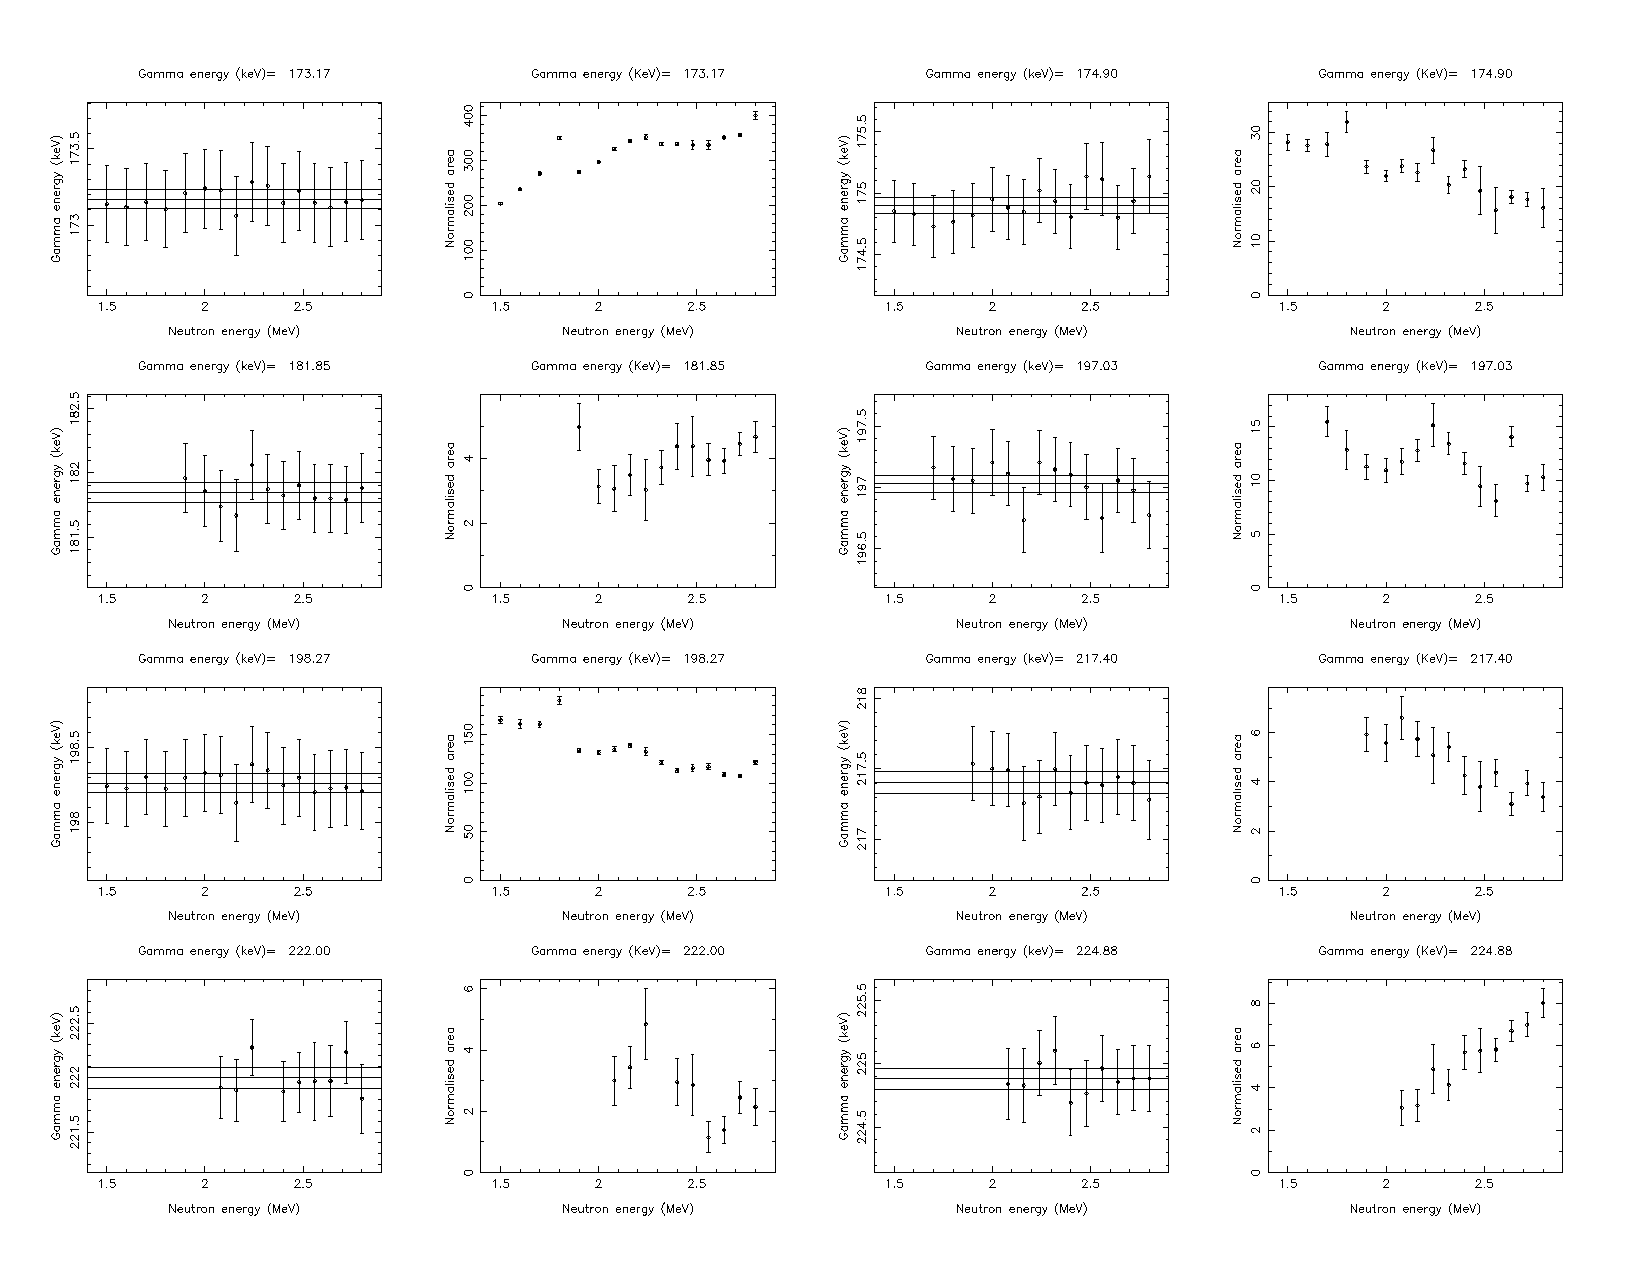
\includegraphics[page=1,angle=90,height=0.95\textheight]{160Gd_ExF_full.pdf}
\end{center}
\begin{center}
\includegraphics[page=2,angle=90,height=0.95\textheight]{160Gd_ExF_full.pdf}
\end{center}
\begin{center}
\includegraphics[page=3,angle=90,height=0.95\textheight]{160Gd_ExF_full.pdf}
\end{center}
\begin{center}
\includegraphics[page=4,angle=90,height=0.95\textheight]{160Gd_ExF_full.pdf}
\end{center}
\begin{center}
\includegraphics[page=5,angle=90,height=0.95\textheight]{160Gd_ExF_full.pdf}
\end{center}
\begin{center}
\includegraphics[page=6,angle=90,height=0.95\textheight]{160Gd_ExF_full.pdf}
\end{center}
\begin{center}
\includegraphics[page=7,angle=90,height=0.95\textheight]{160Gd_ExF_full.pdf}
\end{center}
\begin{center}
\includegraphics[page=8,angle=90,height=0.95\textheight]{160Gd_ExF_full.pdf}
\end{center}
\begin{center}
\includegraphics[page=9,angle=90,height=0.95\textheight]{160Gd_ExF_full.pdf}
\end{center}
\begin{center}
\includegraphics[page=10,angle=90,height=0.95\textheight]{160Gd_ExF_full.pdf}
\end{center}
\begin{center}
\includegraphics[page=11,angle=90,height=0.95\textheight]{160Gd_ExF_full.pdf}
\end{center}
\begin{center}
\includegraphics[page=12,angle=90,height=0.95\textheight]{160Gd_ExF_full.pdf}
\end{center}
\begin{center}
\includegraphics[page=13,angle=90,height=0.95\textheight]{160Gd_ExF_full.pdf}
\end{center}
\begin{center}
\includegraphics[page=14,angle=90,height=0.95\textheight]{160Gd_ExF_full.pdf}
\end{center}
\begin{center}
\includegraphics[page=15,angle=90,height=0.95\textheight]{160Gd_ExF_full.pdf}
\end{center}
\begin{center}
\includegraphics[page=16,angle=90,height=0.95\textheight]{160Gd_ExF_full.pdf}
\end{center}
\begin{center}
\includegraphics[page=17,angle=90,height=0.95\textheight]{160Gd_ExF_full.pdf}
\end{center}
\begin{center}
\includegraphics[page=18,angle=90,height=0.95\textheight]{160Gd_ExF_full.pdf}
\end{center}
\begin{center}
\includegraphics[page=19,angle=90,height=0.95\textheight]{160Gd_ExF_full.pdf}
\end{center}
\begin{center}
\includegraphics[page=20,angle=90,height=0.95\textheight]{160Gd_ExF_full.pdf}
\end{center}
\begin{center}
\includegraphics[page=21,angle=90,height=0.95\textheight]{160Gd_ExF_full.pdf}
\end{center}
\begin{center}
\includegraphics[page=22,angle=90,height=0.95\textheight]{160Gd_ExF_full.pdf}
\end{center}
\begin{center}
\includegraphics[page=23,angle=90,height=0.95\textheight]{160Gd_ExF_full.pdf}
\end{center}
\begin{center}
\includegraphics[page=24,angle=90,height=0.95\textheight]{160Gd_ExF_full.pdf}
\end{center}
\begin{center}
\includegraphics[page=25,angle=90,height=0.95\textheight]{160Gd_ExF_full.pdf}
\end{center}
\begin{center}
\includegraphics[page=26,angle=90,height=0.95\textheight]{160Gd_ExF_full.pdf}
\end{center}
\begin{center}
\includegraphics[page=27,angle=90,height=0.95\textheight]{160Gd_ExF_full.pdf}
\end{center}
\begin{center}
\includegraphics[page=28,angle=90,height=0.95\textheight]{160Gd_ExF_full.pdf}
\end{center}
\begin{center}
\includegraphics[page=29,angle=90,height=0.95\textheight]{160Gd_ExF_full.pdf}
\end{center}
\begin{center}
\includegraphics[page=30,angle=90,height=0.95\textheight]{160Gd_ExF_full.pdf}
\end{center}
\begin{center}
\includegraphics[page=31,angle=90,height=0.95\textheight]{160Gd_ExF_full.pdf}
\end{center}
\begin{center}
\includegraphics[page=32,angle=90,height=0.95\textheight]{160Gd_ExF_full.pdf}
\end{center}
\begin{center}
\includegraphics[page=33,angle=90,height=0.95\textheight]{160Gd_ExF_full.pdf}
\end{center}
\begin{center}
\includegraphics[page=34,angle=90,height=0.95\textheight]{160Gd_ExF_full.pdf}
\end{center}
\begin{center}
\includegraphics[page=35,angle=90,height=0.95\textheight]{160Gd_ExF_full.pdf}
\end{center}


\section{$^{162}$Dy}\label{app:EXF_Dy}
Below are the full excitation function measurements for all $\gamma$-rays observed in the campaign of (n,n$^\prime\gamma$) experiments at the University of Kentucky outlined in \S \ref{sec:Dy_exp}. The complimentary tabulation of the energies of the $\gamma$ rays, the bombarding neutron energy threshold at which the radiation appears, the absolute intensity of $\gamma$ radiation, its origin (whether it is $^{162}$Dy, a background contaminant, etc), and any other notes can be found in Table \ref{tab:162Dy_all_gammas} in the main body of the text.
\begin{center}
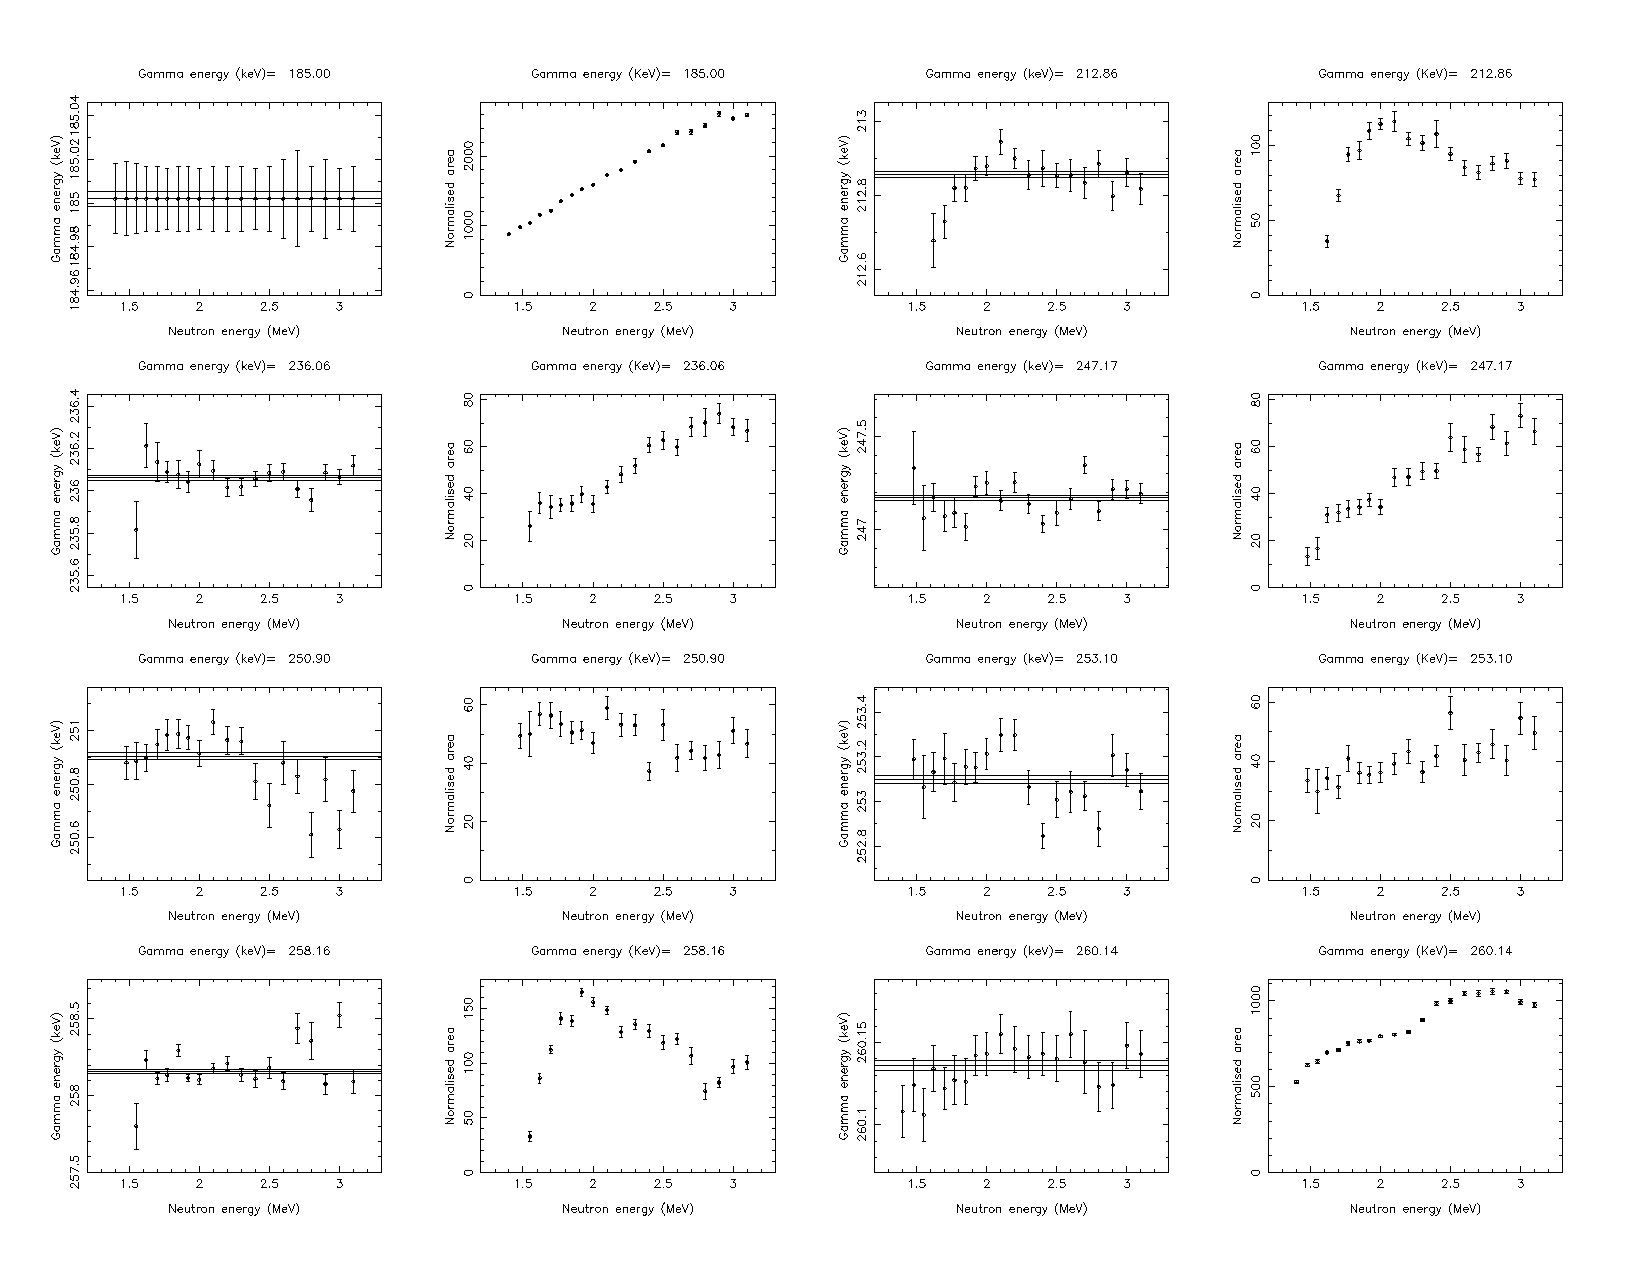
\includegraphics[page=1,angle=90,height=0.95\textheight]{162Dy_stitched.pdf}
\end{center}
\begin{center}
\includegraphics[page=2,angle=90,height=0.95\textheight]{162Dy_stitched.pdf}
\end{center}
\begin{center}
\includegraphics[page=3,angle=90,height=0.95\textheight]{162Dy_stitched.pdf}
\end{center}
\begin{center}
\includegraphics[page=4,angle=90,height=0.95\textheight]{162Dy_stitched.pdf}
\end{center}
\begin{center}
\includegraphics[page=5,angle=90,height=0.95\textheight]{162Dy_stitched.pdf}
\end{center}
\begin{center}
\includegraphics[page=6,angle=90,height=0.95\textheight]{162Dy_stitched.pdf}
\end{center}
\begin{center}
\includegraphics[page=7,angle=90,height=0.95\textheight]{162Dy_stitched.pdf}
\end{center}
\begin{center}
\includegraphics[page=8,angle=90,height=0.95\textheight]{162Dy_stitched.pdf}
\end{center}
\begin{center}
\includegraphics[page=9,angle=90,height=0.95\textheight]{162Dy_stitched.pdf}
\end{center}
\begin{center}
\includegraphics[page=10,angle=90,height=0.95\textheight]{162Dy_stitched.pdf}
\end{center}
\begin{center}
\includegraphics[page=11,angle=90,height=0.95\textheight]{162Dy_stitched.pdf}
\end{center}
\begin{center}
\includegraphics[page=12,angle=90,height=0.95\textheight]{162Dy_stitched.pdf}
\end{center}
\begin{center}
\includegraphics[page=13,angle=90,height=0.95\textheight]{162Dy_stitched.pdf}
\end{center}
\begin{center}
\includegraphics[page=14,angle=90,height=0.95\textheight]{162Dy_stitched.pdf}
\end{center}
\begin{center}
\includegraphics[page=15,angle=90,height=0.95\textheight]{162Dy_stitched.pdf}
\end{center}
\begin{center}
\includegraphics[page=16,angle=90,height=0.95\textheight]{162Dy_stitched.pdf}
\end{center}
\begin{center}
\includegraphics[page=17,angle=90,height=0.95\textheight]{162Dy_stitched.pdf}
\end{center}
\begin{center}
\includegraphics[page=18,angle=90,height=0.95\textheight]{162Dy_stitched.pdf}
\end{center}
\begin{center}
\includegraphics[page=19,angle=90,height=0.95\textheight]{162Dy_stitched.pdf}
\end{center}
\begin{center}
\includegraphics[page=20,angle=90,height=0.95\textheight]{162Dy_stitched.pdf}
\end{center}
\begin{center}
\includegraphics[page=21,angle=90,height=0.95\textheight]{162Dy_stitched.pdf}
\end{center}
\begin{center}
\includegraphics[page=22,angle=90,height=0.95\textheight]{162Dy_stitched.pdf}
\end{center}
\begin{center}
\includegraphics[page=23,angle=90,height=0.95\textheight]{162Dy_stitched.pdf}
\end{center}
\begin{center}
\includegraphics[page=24,angle=90,height=0.95\textheight]{162Dy_stitched.pdf}
\end{center}
\begin{center}
\includegraphics[page=25,angle=90,height=0.95\textheight]{162Dy_stitched.pdf}
\end{center}
\begin{center}
\includegraphics[page=26,angle=90,height=0.95\textheight]{162Dy_stitched.pdf}
\end{center}
\begin{center}
\includegraphics[page=27,angle=90,height=0.95\textheight]{162Dy_stitched.pdf}
\end{center}
\begin{center}
\includegraphics[page=28,angle=90,height=0.95\textheight]{162Dy_stitched.pdf}
\end{center}
\begin{center}
\includegraphics[page=29,angle=90,height=0.95\textheight]{162Dy_stitched.pdf}
\end{center}
\begin{center}
\includegraphics[page=30,angle=90,height=0.95\textheight]{162Dy_stitched.pdf}
\end{center}
\begin{center}
\includegraphics[page=31,angle=90,height=0.95\textheight]{162Dy_stitched.pdf}
\end{center}

